%\documentclass[10pt,notheorems]{beamer}
%\documentclass{beamer} % version for playing slides
\documentclass[handout,10pt]{beamer} % version for print
%\usepackage{xeCJK}
\usepackage{ctex}
%\usepackage{eucal} % for \mathcal
%\usepackage[linewidth=1pt]{mdframed} % for  mdframe environment


 % 1. packages

 % ----------- fonts and symbles ---------
\usepackage{amsmath,amssymb,amsfonts,amsthm}
%\usepackage{CJK}
\usepackage{dsfont}
\usepackage{mathrsfs}
\usepackage{eucal} % for \mathcal

%\renewcommand{\rmdefault}{ptm}


%\usepackage{fontspec}
%\newfontfamily\monaco{Monaco}

%\usepackage{mathbbold} %,bbold

 \usepackage{textcomp} % for \textnormal{\textperthousand}
% -----------------





%\usepackage{slashbox}
%\usepackage[margin=2.2cm]{geometry} % |geometry| package clash with |booktabs| package
%\usepackage{cases}
% -------- tables -------
\usepackage{booktabs} % for \toprule, \bottomrule
\usepackage{tabularx}
\usepackage{multirow}
% --------- figures ---------
\usepackage{graphicx}
% ---------- algorithms -------
\usepackage{algorithm}
\usepackage{algorithmic}
%\usepackage{footnote}
    % |footnote| package occurs error:
    % Runaway argument?
    % \def \insertfootnotetext {\@@ }\def \insertfootnotemark {\@makefnmark \ETC.

\usepackage{listings}

\usepackage[linewidth=1pt]{mdframed} % for  mdframe environment




 \usepackage{color}
 \usepackage{xcolor}     %¸ßÁÁʹÓõÄÑÕÉ«

\usepackage{setspace}
%%\usepackage{type1cm}
\usepackage{adjustbox} % for \adjustbox

\usepackage{accsupp}
\newcommand{\emptyaccsupp}[1]{\BeginAccSupp{ActualText={}}#1\EndAccSupp{}}




%%   figures and tables
\graphicspath{{figure/}}


% 2. new commands

% 2.0 common commands
%\newcommand{\bc}{\begin{center}}
%\newcommand{\ec}{\end{center}}
%\newcommand{\ba}{\begin{array}}
%\newcommand{\ea}{\end{array}}
%\newcommand{\be}{\begin{equation}}
%\newcommand{\ee}{\end{equation}}

% 2.1 colors
\definecolor{dgrey}{rgb}{0.30,0.30,0.30}
\definecolor{lred}{rgb}{0.50,0.00,0.50}
\definecolor{lblue}{rgb}{0.8,0.8,1}
\definecolor{dred}{rgb}{0.6,0,0}
\definecolor{dblue}{rgb}{0,0,0.5}
\definecolor{dgrey}{rgb}{0.35,0.35,0.35}
\definecolor{rred}{rgb}{0.9,0,0}
\definecolor{mylblue}{rgb}{0.3,0.2, 0.8}

\definecolor{commentcolor}{RGB}{85,139,78}
\definecolor{stringcolor}{RGB}{206,145,108}
\definecolor{keywordcolor}{RGB}{34,34,250}
\definecolor{backcolor}{RGB}{220,220,220}

\newcommand{\blue}[1]{{\color{blue}#1}}
\newcommand{\dblue}[1]{{\color{dblue}#1} }
\newcommand{\red}[1]{{\color{red}#1}}
\newcommand{\dred}[1]{{\color{dred}#1}}
\newcommand{\cyan}[1]{{\color{cyan}#1}}
\newcommand{\bfblue}[1]{\textbf{\color{dblue}#1} }
\newcommand{\bfred}[1]{\textbf{\color{dred}#1} }
\newcommand{\green}[1]{{\color{green}#1}}
%\newcommand{\alert}[1]{{\color{red}#1}}
\newcommand{\black}[1]{{\color{black}#1}}
\newcommand{\light}[1]{{\color{blue}\textbf{#1}}}
\newcommand{\hot}[1]{{\color{dred}#1}}
 \newcommand{\highlight}[1]{ \textbf{\color{mylblue}#1}}
 \newcommand{\important}[1]{{\color{red}#1}} % for highlighting  some words

 \newcommand{\mystar}{\dred{$^{\clubsuit}$ }}
  \newcommand{\doublestar}{\dred{$^{\clubsuit\clubsuit}$ }}

\newcommand{\mynote}[1]{{\footnotesize \color{mylblue}#1}}

 \newcommand{\hint}[1]{{\small \color{mylblue}#1}}
\newcommand{\smallhint}[1]{{\small \color{dgrey}#1}}
\newcommand{\footnotehint}[1]{{\footnotesize \color{dgrey}#1}}
\newcommand{\tinyhint}[1]{{\tiny \color{dgrey}#1}}
\newcommand{\mytitle}[1]{\medskip{\large \textbf{\color{mylblue}#1}}}
\newcommand{\normaltitle}[1]{\medskip{ \textbf{\color{mylblue}#1}}}

%\newcommand{\head}[1]{\textbf{\large\color{blue}#1}}
%\newcommand{\heading}[1]{\textbf{\large\color{blue}#1}}

\newcommand{\myfbox}[2]{ \bigskip \begin{center} \fbox{\parbox{#1}{ #2  }} \end{center}\bigskip }

\newcommand{\myvar}[1]{}
%\newcommand{\mynote}[1]{#1}

% 2.2 mathematical symbols

\newcommand{\drightarrow}{\stackrel{d.}{\rightarrow}}
\newcommand{\prightarrow}{\stackrel{p.}{\rightarrow}}
\newcommand{\bernoulli}{\textnormal{Ber}}
\newcommand{\cov}{\mathsf{Cov}}
\newcommand{\corr}{\mathbf{Corr}}
\newcommand{\regret}{\textnormal{Regret}}
\newcommand{\conv}{\textnormal{conv}}
\newcommand{\dotdiv}{\stackrel{\centerdot}{-}}
\newcommand{\dom}{\textnormal{dom}}
\newcommand{\convergenceinprob}{\stackrel{P}{\rightarrow}}
\newcommand{\convergenceindist}{\rightsquigarrow}
\newcommand{\probability}{\mathbb{P}}
\newcommand{\expectation}{\mathbb{E}}
\newcommand{\epi}{\textnormal{epi}}
\newcommand{\variance}{\mathbb{V}}
\newcommand{\var}[1]{\mathbb{V}(#1)}
\newcommand{\covariance}{\mathsf{Cov}}
\newcommand{\empiricalrisk}[1]{\hat{R}(#1)}
\newcommand{\expectedrisk}[1]{R(#1)}
\newcommand{\mgf}[1]{\psi_{#1}(\lambda)}
\newcommand{\mgfexpansion}[1]{\expectation[e^{\lambda#1}]}
\newcommand{\mgfmultivariate}[1]{\expectation[e^{\lambda^\transpose#1}]}
\newcommand{\transpose}{{\mathsf{T}}}
\newcommand{\real}{\mathbb{R}}
\newcommand{\gaussian}[2]{\mathcal{N}(#1,#2)}
\newcommand{\subGaussian}[1]{\mathsf{subG}(#1)}
\newcommand{\indicator}[1]{\mathbb{I}[#1]}
\newcommand{\x}[1]{x^{(#1)}}
\newcommand{\y}[1]{y^{(#1)}}
\newcommand{\z}[1]{z^{(#1)}}
\newcommand{\feature}{x}
\newcommand{\response}{y}
\newcommand{\supofempiricalprocess}{\|\mathbb{P}_n-\mathbb{P}\|_{\decisionspace}}
\newcommand{\decisionspace}{\mathscr{F}}
\newcommand{\decisionfunction}{f}
\newcommand{\featurespace}{\mathcal{X}}
\newcommand{\classifierestimate}{\widehat{h}}
\newcommand{\classifiertrue}{h^\star}
\newcommand{\classifier}{h}
\newcommand{\hypothesisclass}{\mathcal{H}}
\newcommand{\dataset}{\mathcal{D}}
\newcommand{\defineas}{\stackrel{\textnormal{def}}{=}}
\newcommand{\rademachercomplexity}[1]{\mathsf{Rad}_n\left(#1\right)}
\newcommand{\loss}{\ell}
\newcommand{\composite}{\circ}
\newcommand{\convexhull}{\mathsf{conv}}
\newcommand{\norm}[2][2]{\|#2\|_{#1}}
\newcommand{\shatteringcoefficient}[2]{\mathcal{S}(#1,#2)}
\newcommand{\vcdimension}[1]{\mathsf{VC}\left(#1\right)}
\newcommand{\rank}{\mathsf{rank}}
\newcommand{\innerproduct}[2]{\left\langle #1, #2\right\rangle}
\newcommand{\modelparameter}{\theta}
\newcommand{\ball}[3][]{\mathcal{B}_{{#1}}\left(#2,#3\right)}
\newcommand{\metric}{d}
\newcommand{\coveringnumber}[4][]{N_{{#1}}\left(#2,#3,#4\right)}
\newcommand{\trace}{\textnormal{tr}}
\newcommand{\std}{\textnormal{std}}
\newcommand{\sgn}{\textnormal{sign}}
%\renewcommand{\span}{\textnormal{span}}

 % do not overwrite the existing command \span
 % as it leads to an error of
 %  "Missing # Inserted in Alignment Preamble" for ``align'' environment

\newcommand{\myspan}{\textnormal{span}}

%%%
\newcommand{\rightarrowd}{\stackrel{d}{\rightarrow}}
\newcommand{\rightarrowp}{\stackrel{p}{\rightarrow}}
\newcommand{\defeq}{ \stackrel{\textnormal{def}}{=}}
\newcommand{\proj}{ \textnormal{Proj}}
\newcommand{\dist}{\textnormal{dist}}

\newcommand{\argmax}{\textnormal{argmax}}
\newcommand{\argmin}{\textnormal{argmin}}
\newcommand{\subg}{\textnormal{subG}}


 \newcommand{\bba}{\mathbb{A}}
\newcommand{\bbb}{\mathbb{B}}
\newcommand{\bbc}{\mathbb{C}}
\newcommand{\bbd}{\mathbb{D}}
\newcommand{\bbe}{\mathbb{E}}
\newcommand{\bbf}{\mathbb{F}}
\newcommand{\bbg}{\mathbb{G}}
\newcommand{\bbh}{\mathbb{H}}
\newcommand{\bbi}{\mathbb{I}}
\newcommand{\bbj}{\mathbb{J}}
\newcommand{\bbk}{\mathbb{K}}
\newcommand{\bbl}{\mathbb{L}}
\newcommand{\bbm}{\mathbb{M}}
\newcommand{\bbn}{\mathbb{N}}
\newcommand{\bbo}{\mathbb{O}}
\newcommand{\bbp}{\mathbb{P}}
\newcommand{\bbq}{\mathbb{Q}}
\newcommand{\bbr}{\mathbb{R}}
\newcommand{\bbs}{\mathbb{S}}
\newcommand{\bbt}{\mathbb{T}}
\newcommand{\bbu}{\mathbb{U}}
\newcommand{\bbv}{\mathbb{V}}
\newcommand{\bbw}{\mathbb{W}}
\newcommand{\bbx}{\mathbb{X}}
\newcommand{\bby}{\mathbb{Y}}
\newcommand{\bbz}{\mathbb{Z}}

\newcommand{\bfa}{\mathbf{a}}
\newcommand{\bfb}{\mathbf{b}}
\newcommand{\bfc}{\mathbf{c}}
\newcommand{\bfd}{\mathbf{d}}
\newcommand{\bfe}{\mathbf{e}}
\newcommand{\bff}{\mathbf{f}}
\newcommand{\bfg}{\mathbf{g}}
\newcommand{\bfh}{\mathbf{h}}
\newcommand{\bfi}{\mathbf{i}}
\newcommand{\bfj}{\mathbf{j}}
\newcommand{\bfk}{\mathbf{k}}
\newcommand{\bfl}{\mathbf{l}}
\newcommand{\bfm}{\mathbf{m}}
\newcommand{\bfn}{\mathbf{n}}
\newcommand{\bfo}{\mathbf{o}}
\newcommand{\bfp}{\mathbf{p}}
\newcommand{\bfq}{\mathbf{q}}
\newcommand{\bfr}{\mathbf{r}}
\newcommand{\bfs}{\mathbf{s}}
\newcommand{\bft}{\mathbf{t}}
\newcommand{\bfu}{\mathbf{u}}
\newcommand{\bfv}{\mathbf{v}}
\newcommand{\bfw}{\mathbf{w}}
\newcommand{\bfx}{\mathbf{x}}
\newcommand{\bfy}{\mathbf{y}}
\newcommand{\bfz}{\mathbf{z}}

\newcommand{\bfA}{\mathbf{A}}
\newcommand{\bfB}{\mathbf{B}}
\newcommand{\bfC}{\mathbf{C}}
\newcommand{\bfD}{\mathbf{D}}
\newcommand{\bfE}{\mathbf{E}}
\newcommand{\bfF}{\mathbf{F}}
\newcommand{\bfG}{\mathbf{G}}
\newcommand{\bfH}{\mathbf{H}}
\newcommand{\bfI}{\mathbf{I}}
\newcommand{\bfJ}{\mathbf{J}}
\newcommand{\bfK}{\mathbf{K}}
\newcommand{\bfL}{\mathbf{L}}
\newcommand{\bfM}{\mathbf{M}}
\newcommand{\bfN}{\mathbf{N}}
\newcommand{\bfO}{\mathbf{O}}
\newcommand{\bfP}{\mathbf{P}}
\newcommand{\bfQ}{\mathbf{Q}}
\newcommand{\bfR}{\mathbf{R}}
\newcommand{\bfS}{\mathbf{S}}
\newcommand{\bfT}{\mathbf{T}}
\newcommand{\bfU}{\mathbf{U}}
\newcommand{\bfV}{\mathbf{V}}
\newcommand{\bfW}{\mathbf{W}}
\newcommand{\bfX}{\mathbf{X}}
\newcommand{\bfY}{\mathbf{Y}}
\newcommand{\bfZ}{\mathbf{Z}}


\newcommand{\bfSigma}{\mathbf{\Sigma}}
\newcommand{\bfrho}{\mathbf{\rho}}

\newcommand{\cala}{\mathcal{A}}
\newcommand{\calb}{\mathcal{B}}
\newcommand{\calc}{\mathcal{C}}
\newcommand{\cald}{\mathcal{D}}
\newcommand{\cale}{\mathcal{E}}
\newcommand{\calf}{\mathcal{F}}
\newcommand{\calg}{\mathcal{G}}
\newcommand{\calh}{\mathcal{H}}
\newcommand{\cali}{\mathcal{I}}
\newcommand{\calj}{\mathcal{J}}
\newcommand{\calk}{\mathcal{K}}
\newcommand{\call}{\mathcal{L}}
\newcommand{\calm}{\mathcal{M}}
\newcommand{\caln}{\mathcal{N}}
\newcommand{\calo}{\mathcal{O}}
\newcommand{\calp}{\mathcal{P}}
\newcommand{\calq}{\mathcal{Q}}
\newcommand{\calr}{\mathcal{R}}
\newcommand{\cals}{\mathcal{S}}
\newcommand{\calt}{\mathcal{T}}
\newcommand{\calu}{\mathcal{U}}
\newcommand{\calv}{\mathcal{V}}
\newcommand{\calw}{\mathcal{W}}
\newcommand{\calx}{\mathcal{X}}
\newcommand{\caly}{\mathcal{Y}}
\newcommand{\calz}{\mathcal{Z}}


% 3. theorem and environments

%\newtheorem{theorem}{Theorem}%[section]
\newtheorem{proposition}{Proposition}%[section]
%\newtheorem{property}{Property}%[section]
%\newtheorem{lemma}{Lemma}%[section]
%\newtheorem{corollary}{Corollary}%[section]
%\newtheorem{definition}{Definition}%[section]
%\newtheorem{example}{Example}%[section]
%\newtheorem{remark}{Remark}%[section]
%\newtheorem{note}{Note}%[section]
%\newtheorem{problem}{Problem}%[section]
\newtheorem{exercise}{Exercise}
%\newtheorem{assumption}{Assumption}
\newtheorem*{lemma_star}{Lemma}
\newtheorem*{theorem_star}{Theorem}

%\newenvironment{summary}[1][Summary]{\par\medskip   \color{dred}\textbf{\large#1. } }{ \medskip}
%\newenvironment{remark}[1][Remark]{\par\medskip  \begin{small} \color{dblue}\textbf{#1. } }{ \end{small}\medskip}
%\renewenvironment{proof}[1][Proof]{\noindent\textbf{#1.} }{\mbox{} \hfill{\small\textrm{$\Box$}}\vspace{1ex}}
% \newenvironment{answer}[1][Answer]{\par\medskip \color{dblue}\textbf{\large#1. }}{ \medskip}

\newenvironment{summary}[1][总结]{\par\medskip   \color{dred}\textbf{\large#1 } }{ \medskip}
\newenvironment{remark}[1][注意]{\par\medskip   \color{dblue}\textbf{\large#1 } }{ \medskip}
\newenvironment{footnoteremark}{ \color{dblue}\begin{footnotesize} }{\end{footnotesize}}
\renewenvironment{proof}[1][证明]{\noindent\textbf{#1.} }{\mbox{} \hfill{\small\textrm{$\Box$}}\vspace{1ex}}
 \newenvironment{question}[1][Q.]{\par\medskip {\color{lred}\large#1}}{ \medskip}
 \newenvironment{answer}[1][Answer]{\par\medskip \color{dblue}\textbf{\large#1 }}{ \medskip}

% 4. beamer setting




%\newtheorem{definition}{\textbf{¶¨Òå}}[section]
%\newtheorem{proposition}[definition] { \textbf{ÃüÌâ}}
%\newtheorem{lemma}[definition] { \textbf{ÒýÀí}}
%\newtheorem{theorem}[definition]{ \textbf{¶¨Àí}}
%\newtheorem{corollary}[definition] { \textbf{ÍÆÂÛ}}
%\newtheorem{remark}[definition] { \textbf{×¢}}
%\newtheorem{example}[definition] { \textbf{Àý}}

%\newcommand{\shadow}[1]{\begin{center}
%\bf{\textcolor{dblue}{\shadowbox{\parbox{3.8in}
% {\textcolor{red}
% {\vspace{1mm}#1}}}}}
%\end{center}}
%
%\newcommand{\head}[1]{\begin{center}
%\bf{\textcolor{dblue}{\shadowbox{\parbox{3.8in}
% {\textcolor{dred}
% {\vspace{1mm}#1}}}}}
%\end{center}}
%
%
%\newcommand{\heading}[1]{%
%  \begin{center}
%    \large\bf
%    \shadowbox{#1}%
%  \end{center}
%\vspace{1ex minus 1ex}}

% set  space above and below math equations in display style

\expandafter\def\expandafter\normalsize\expandafter{%
    \normalsize
    \setlength\abovedisplayskip{1.5ex}
    \setlength\belowdisplayskip{1.2ex}
    \setlength\abovedisplayshortskip{0.5ex}
    \setlength\belowdisplayshortskip{0.5ex}
}

% Ìí¼ÓÒ³Âë´úÂ룬¹È¸èÕÒµ½µÄ¡£
\addtobeamertemplate{navigation symbols}{}{%
    %\usebeamerfont{footline}%
    %\usebeamercolor[fg]{footline}%
    \setbeamercolor{footline}{fg=blue}
    \setbeamerfont{footline}{series=\bfseries}
    \hspace{1em}%
    \normalsize{\insertframenumber/\inserttotalframenumber}
}

% section numbering
\setbeamertemplate{section in toc}[sections numbered]
\setbeamertemplate{subsection in toc}[subsections numbered]



\lstset{                        %¸ßÁÁ´úÂëÉèÖÃ
%basicstyle=\small, % print whole listing small
%basicstyle=\footnotesize\sffamily, % print whole listing small
basicstyle=\footnotesize\rmfamily, % print whole listing small
%basicstyle=\rmfamily, % print whole listing small
    language=python,                    %PythonÓï·¨¸ßÁÁ
    %linewidth=0.9\linewidth,            %Áбílist¿í¶È
    %basicstyle=\ttfamily,              %ttÎÞ·¨ÏÔʾ¿Õ¸ñ
    commentstyle=\color{commentcolor},  %×¢ÊÍÑÕÉ«
    keywordstyle=\color{keywordcolor},  %¹Ø¼ü´ÊÑÕÉ«
    stringstyle=\color{stringcolor},    %×Ö·û´®ÑÕÉ«
    %showspaces=true,                   %ÏÔʾ¿Õ¸ñ
    numbers=left,                       %ÐÐÊýÏÔʾÔÚ×ó²à
    %numberstyle=\tiny\emptyaccsupp,     %ÐÐÊýÊý×Ö¸ñʽ
    numberstyle=\tiny,                  %ÐÐÊýÊý×Ö¸ñʽ
    numbersep=5pt,                      %Êý×Ö¼ä¸ô
    frame=single,                       %¼Ó¿ò
    framerule=0pt,                      %²»»®Ïß
    %escapeinside=@@,                    %ÌÓÒݱêÖ¾
    escapeinside=``,                    %ÌÓÒݱêÖ¾
    emptylines=1,                       %
    xleftmargin=3em,                    %list×ó±ß¾à
    backgroundcolor=\color{backcolor},  %ÁÐ±í±³¾°É«
    tabsize=4,                          %ÖƱí·û³¤¶ÈΪ4¸ö×Ö·û
    %gobble=4                            %ºöÂÔÿÐдúÂëÇ°4¸ö×Ö·û
    breaklines=true,
    extendedchars=false
    }

\lstdefinestyle{numbers}{numbers=left, stepnumber=1, numberstyle=\tiny, numbersep=10pt}
 \lstdefinestyle{nonumbers}{numbers=none}

\newcommand{\alertcode}[1]{{\color{red}#1}} % used for alerting codes

%\lstset{numbers=left, numberstyle=\tiny,
%keywordstyle=\color{blue!70},
%commentstyle=\color{red!50!green!50!blue!50},
%frame=shadowbox,
%rulesepcolor=\color{red!20!green!20!blue!20},
%escapeinside=``,
%framesep = 2ex,
%rulesep = 1ex
%%framexrightmargin= 1em %
%}


% Vary the color applet  (try out your own if you like)
\colorlet{structure}{red!65!black}

%\beamertemplateshadingbackground{yellow!50}{white}


%\setbeamerfont{normal text}{family=\rmfamily}
%\setbeamerfont{frametitle}{family=\rmfamily}

% Changing the fonts: this will make the slides more readable and the math look like regular tex math
\usefonttheme{serif}



% set spaces

\setstretch{1.2}  % ÉèÖÃÐоà

\addtobeamertemplate{block begin}{\setlength\abovedisplayskip{0pt}} % reduce the large space before a block

% set section number styles



\newcommand{\secno}{Sec.\,\thesection\ }
\newcommand{\subsecno}{Sec.\,\thesubsection\ }

% set logo

 \pgfdeclareimage[width=1.0]{small-logo}{SMaLL.jpg}
%
 \logo{\vbox{\vskip0.1 \hbox{\pgfuseimage{small-logo}}}}

% set math equation fontsize

 \makeatletter
\DeclareMathSizes{\f@size}{10}{5}{5}
\makeatother

% for chinese section name
\hypersetup{CJKbookmarks=true}


% Vary the color applet  (try out your own if you like)
\colorlet{structure}{red!65!black}

%\beamertemplateshadingbackground{yellow!50}{white}
\pgfdeclareimage[ width=1.0cm]{small-logo}{small-member/SMaLL}

\logo{\vbox{\vskip0.1cm\hbox{\pgfuseimage{small-logo}}}}




\begin{document}
%\begin{CJK}{GBK}{song}
%\begin{CJK*}{GBK}{kai}

\addtobeamertemplate{block begin}{\setlength\abovedisplayskip{0pt}} % reduce the large space before a block




\title[数值优化]{第5章4-5节 牛顿法、拟牛顿法}

\bigskip

\author[]{
		 \underline{SMaLL} 
	}
	
\institute[CUP]{
		\inst{1}
		中国石油大学(华东)\\
		SMaLL 课题组   \\
		\blue{small.sem.upc.edu.cn}\\
		liangxijunsd@163.com \\ 
	 
}
		
\date[2023]{\small    2023}



\subject{Numerical optimization}

%\pgfdeclaremask{fsu}{fsu_logo_ybkgrd}
%\pgfdeclareimage[mask=fsu,width=1cm]{fsu-logo}{fsu_logo_ybkgrd}

%\logo{\vbox{\vskip0.1cm\hbox{\pgfuseimage{fsu-logo}}}}

  \frame
  {
    \titlepage
  }

%\frame{
%    \frametitle{纲要}
%    \tableofcontents[hideallsubsections]% 显示在目录中加亮的当前章节
%  }

%%
%% 定义框架页
%%
\AtBeginSection[]{                              % 在每个Section前都会加入的Frame
  \frame<handout:1>{   
    \frametitle{纲要}
    %\tableofcontents[current,currentsubsection] % 显示在目录中加亮的当前章节
    \tableofcontents[hideallsubsections,current] % 显示在目录中加亮的当前章节
  }
}
%\AtBeginSubsection[]                            % 在每个子段落之前
%{
%  \frame<handout:1>                             % handout:0 表示只在手稿中出现
%  {
%    \frametitle{Table of Contents}
%    \tableofcontents[current,currentsubsection] % 显示在目录中加亮的当前章节
%  }
%}




%\begin{frame}
%%  \frametitle{研究课题}
%\frametitle{纲要}
%
% \vspace{3ex}
%
%\begin{large}
%\begin{itemize}
%
%  \item Online Convex Optimization
%
%  \vspace{3ex}
%  \item Online Learning
%
%  \vspace{3ex}
%  \item Online Learning Framework for C-Ranker
%
%\end{itemize}
%\end{large}
%
%\vspace{5ex}
%
%\mbox{}
%
%\end{frame}






\section{牛顿法} \label{sec_1_2_4}


\begin{frame}[fragile]
\frametitle{牛顿法求解非线性方程}

牛顿法:可用于一元函数求根 

\begin{itemize}
\item<1-> 设 $\phi(t):R\rightarrow R$. 考虑等式
$$
    \phi(t) = 0.
$$
\item<only@2-3> 牛顿法基于线性近似的思想
$$
    \phi(t+\Delta t) = \phi(t) + \phi'(t) \Delta t + o(|\Delta t|).
$$
$\Rightarrow$  因此方程  $\phi(t + \Delta t) = 0$ 可以由以下线性方程近似:
$$
    \phi(t) + \phi'(t) \Delta t = 0.
$$
  % end blue

\item<3-> 
\begin{minipage}{0.5\textwidth}
\hint{ 这个等式的解是最优位移 $\Delta t^* = t^* -t$  的近似 }
\red{ $\rightarrow$ 算法形式:
$$
    t_{k+1}^{} = t_k - \frac{\phi(t_k)}{\phi'(t_k)}
$$
}
\end{minipage}
 \begin{minipage}{0.4\textwidth}
\begin{center}
 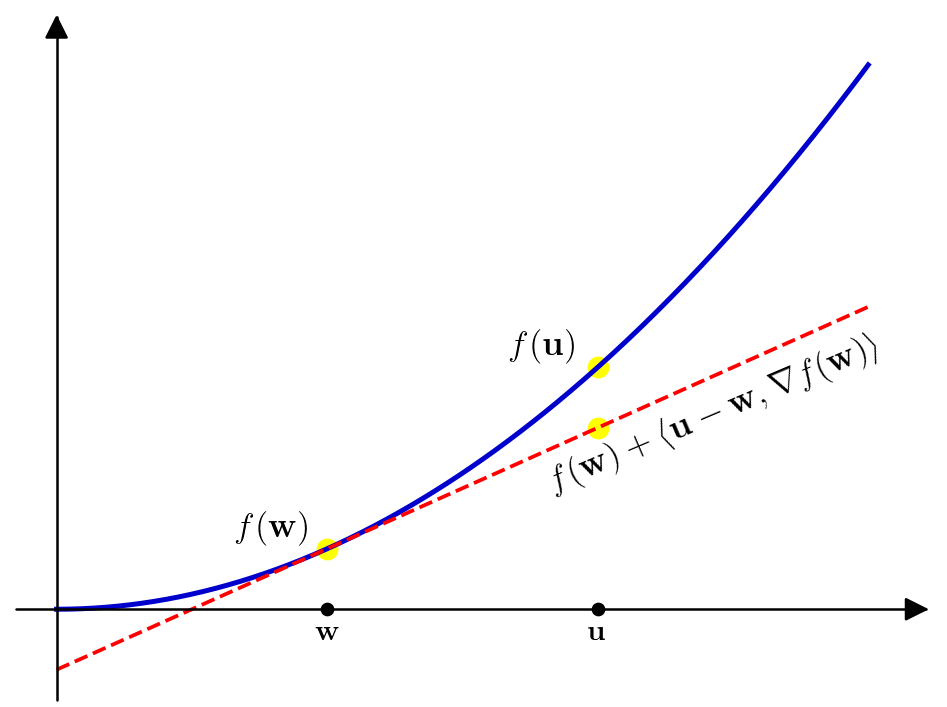
\includegraphics[width=1.0\textwidth]{figure/newton fig1.png}
 \end{center}
\end{minipage}

\end{itemize}

%


  %%%



  %%%



\end{frame}

\begin{frame}[fragile]
\frametitle{牛顿法求解非线性方程}


 求解非线性方程组,
$$
    F(x) = 0,
$$
其中 $x \in R^n$ 且 \blue{$F(x): R^n \rightarrow R^n$}.

\begin{itemize}
  \item
   $\Delta x$: 线性方程组的一种解法:
\red{
$$
    F(x) + \nabla F(x)_{}^{T} \Delta x = 0,
$$
(它称为牛顿方程),
} %
\footnotehint{
其中 $\nabla F(x) = [\nabla f_1(x) \cdots \nabla f_n(x)] \in R_{}^{n \times n}$,
$$
    F(x) = \left[\begin{array}{c}
     f_1(x) \\
     f_2(x)\\
     \vdots \\
     f_n(x)\\
     \end{array}
     \right].
$$
}
\item
\textbf{备注:}
\footnotehint{
 牛顿方程还可写为
$
    F(x) + J F(x)_{}^{} \Delta x = 0,
$
其中 $J F(x) = \nabla F(x)_{}^{T}$ 是雅可比行列式.
{如果  $JF(x)$ 是非退化的,}
$$
    x_{k+1}^{} = x_{k} - [JF(x_k)]_{}^{-1}F(x_k).
$$
}

\end{itemize}




\end{frame}

\begin{frame}[fragile]
\frametitle{牛顿法求解无约束极小化问题}



  无约束极小化问题 $\min_x f(x)$
$\longrightarrow$ 可以转化为非线性方程求根问题
\begin{equation}\label{EQ_1_2_20}
    f'(x) = 0.
\end{equation}
\footnotehint{
    (虽然这种转化与原问题并不完全等价,但它在非退化情况下是有效的.)
}
  应用牛顿法 $\rightarrow$
得到如下牛顿方程:
$$
    f'(x) + f''(x)\Delta x = 0.
$$
 无约束问题的牛顿法表示为:
\dred{
\begin{equation}\label{EQ_1_2_21}
        x_{k+1}^{} = x_k - [f''(x_k)]_{}^{-1} f'(x_k).
\end{equation}
}


\end{frame}

\begin{frame}[fragile]
\frametitle{利用二次逼近的思想求牛顿法}

 利用\hint{二次近似}的思想,关于点$x_k$:
$$
    \phi(x) = f(x_k) + \langle f'(x_k),x-x_k\rangle + \frac{1}{2} \langle f''(x_k)(x-x_k), x-x_k\rangle.
$$
假设 $f''(x_k) \succ 0$. 我们可以选择二次函数$\phi(x)$的最小值点作为下个迭代点 $x_{k+1}^{}$ . 这意味着
$$
    \phi'(x_{k+1}^{}) = f'(x_k) + f''(x_k) (x_{k+1}^{} - x_k) = 0,
$$
$\Rightarrow$再次得到牛顿迭代公式 (\ref{EQ_1_2_21}): $x_{k+1}^{} = x_k - [f''(x_k)]_{}^{-1} f'(x_k)$.


\end{frame}

\begin{frame}[fragile]
\frametitle{牛顿法的优缺点}


\begin{itemize}
  \item \hint{优点:}   牛顿法在严格局部极小值附近的收敛速度非常快.

  \item \hint{缺点:}
\begin{enumerate}
\item 如果 $f''(x_k)$ 是奇异阵,那么该方法将无法使用.
\item 牛顿迭代过程可能不收敛.
\end{enumerate}
\end{itemize}

\end{frame}

\begin{frame}[fragile]
\frametitle{示例}

\begin{example}[示例]\label{eg_1_2_4}
\textbf{[牛顿迭代过程可能不收敛]}
用牛顿法求下列一元函数的零点:
$$
    \phi(t) = \frac{t}{\sqrt{1+t^2}}.
$$
注意到,有唯一的零点 $t^* = 0$. 同时有
$
    \phi'(t) = \frac{1}{(1 + t^2)^{3/2}}.
$
牛顿迭代过程如下:
$$
    t_{k+1}^{} = t_k - \frac{\phi(t_k)}{\phi'(t_k)}  = t_k - \frac{t_k}{\sqrt{1+t_k^2}}\cdot [1+t_k^2]^{3/2} = -t_k^3.
$$
因此,
\begin{itemize}
\item 若 $|t_0|<1$, 那么该方法收敛,且收敛速度非常快.
\item 若 $t_0 = \pm 1$ 是这个方法的 \hint{震荡点}
\item 若 $|t_0|>1$, 该方法将 \hint{不收敛}
\end{itemize}
\end{example}


\footnotehint{函数 $
    \phi(t) = \frac{t}{\sqrt{1+t^2}}.
$
是由
$
    f(t)  = \sqrt{1+t^2}.
$派生函数}
\end{frame}

\begin{frame}[fragile]
\frametitle{阻尼牛顿法}



为了避免不收敛的问题,可以应用\hint{阻尼牛顿法}:
\begin{center}
\fbox{
$
    x_{k+1}^{} = x_k - \dred{h_k} [f''(x_k)]_{}^{-1} f'(x_k),
$
}
\end{center}
其中$h_k >0$ 是步长参数.

\begin{itemize}
  \item
在方法的初始阶段,我们可以使用与梯度下降法相同的步长策略.

\item 在最后阶段,可以选择 $h_k = 1$.

\end{itemize}



\end{frame}

\begin{frame}[fragile]
\frametitle{牛顿法的局部收敛性}


接下来研究牛顿方法的局部收敛性。
考虑问题
$$
    \min_{x\in R^n}^{} \ f(x)
$$
满足以下假设:

\begin{enumerate}
    \item $f\in C_{M}^{2,2}(R^n)$,且Hessian矩阵Lipschitz连续,Lipschitz常数为M>0.
    \item 具有正定的Hessian矩阵$f$,$f$在$x^*$处存在局部极小点:
    \begin{equation}\label{EQ_1_2_22}
        f''(x^*) \succeq lI_n, l>0.
        \end{equation}
    \item 初始点 $x_0$ 离 $x^*$足够近.
\end{enumerate}



\end{frame}

\begin{frame}[fragile]
\frametitle{牛顿方法的局部收敛性:准备工作}

\begin{corollary}[推论]\label{coro_1_2_2}\tinyhint{[Nesterov. Intro. Lec. on Convex Opt. pp.24, Coro.1.2.2]}

    设 $f \in C_M^{2,2}(R^n)$ 且 $ \|y-x\| =r$, 因此
    $$
        f''(x) - MrI_n \preceq f''(y) \preceq f''(x)+ MrI_n
    $$
\end{corollary}


%\framebreak
\end{frame}

\begin{frame}[allowframebreaks]
\frametitle{牛顿方法的局部收敛性:分析}
考虑迭代过程: $x_{k+1}^{} = x_k - [f''(x_k)]_{}^{-1}f'(x_k)$.
然后使用与梯度法相同的推理,我们得到:
$$
\begin{aligned}
    x_{k+1}-x^*     &  =  x_k - x^* - [f''(x_k)]_{}^{-1} f'(x_k) \\
            &    = x_k - x^* - [f''(x_k)]_{}^{-1} \int_0^1 f''(x^* + \tau(x_k-x^*))(x_k-x^*) d\tau \\
            & = [f''(x_k)]_{}^{-1} G_k (x_k - x^*),
\end{aligned}
$$
其中 $G_k = \int_0^1 [f''(x_k) - f''(x^* +\tau (x_k-x^*))]d\tau$.

记 $r_k = \|x_k - x^*\|$. 则
$$
\begin{aligned}
    \|G_k\| &  = \| \int_0^1 [f''(x_k) - f''(x^* +\tau (x_k-x^*))]d\tau \| \\
            &  \leq   \int_0^1 \| f''(x_k) - f''(x^* +\tau (x_k-x^*))] \| d\tau  \\
            & \leq \int_0^1 M(1-\tau) r_k d\tau  = \frac{r_k}{2}M. \\
\end{aligned}
$$
由定理 \ref{coro_1_2_2},和 (\ref{EQ_1_2_22}),得到
$$
    f''(x_k) \succeq f''(x^*) - Mr_k I_n \succeq (l-Mr_k) I_n.
$$
因此,若 $r_k < \frac{l}{M}$, 则 $f''(x_k)$ 是正定的且
$$
    \| [f''(x_k)]_{}^{-1}\| \leq (l - M r_k )_{}^{-1}.
$$
对于足够小的 $r_k$  ($r_k < \frac{2l}{3M}$), 有
$$
   \blue{ r_{k+1} \leqslant \frac{M\left(r_k\right)^2}{2\left(l-M r_k\right)}<r_k.}
$$
\dred{这种类型的收敛速度叫做二次收敛}


\footnotehint{
$$
\frac{M\left(r_k\right)^2}{2\left(l-M r_k\right)}<r_k\ \Longleftrightarrow M r_k < 2(l-M\cdot r_k) \ \Longleftrightarrow r_k < \frac{2l}{3M}.
$$
}

\end{frame}

\begin{frame}[fragile]
\frametitle{牛顿法的局部收敛性}

%Thus, we have proved the following theorem.
\begin{theorem}[定理]\label{TH_1_2_5}
    若函数 $f(x)$ 满足我们的假设.
   且初始点 $x_0$ 足够接近 $x^*$:
    $$
        \|x_0 - x^* \|  < \bar{r} = \frac{2l}{3M}.
    $$
   那么对于所有的 $k$ ,$\|x_k -x^*\| < \bar{r}$ 且牛顿法二次收敛
    $$
   \blue{ \|x_{k+1}^{}-x^*\| \leq \frac{M \|x_k -x^*\|^2}{2(l-M \|x_k - x^*\|)}. }
$$
\end{theorem}


\footnotehint{
\begin{itemize}
\item
与梯度下降法的收敛速度进行比较
  $\rightarrow$
牛顿法要快得多.

\item 牛顿法\hint{迭代点列的区域}几乎与梯度下降迭代法点列的收敛区域相同


\item $\rightarrow$可在算法的初始阶段使用梯度下降法的迭代格式 $\rightarrow$  接近局部极小解
$\rightarrow$
在算法的最后阶段 用牛顿法来完成迭代
\end{itemize}
}



\end{frame}

\begin{frame}[fragile]
\frametitle{收敛速度和复杂性界限}


 \only<1>{收敛速度和算法复杂度的界互为反函数.}

\begin{enumerate}
\item<only@1> \textbf{次线性速率.} 次线性速率常用\blue{迭代次数的幂函数来描述.}
  比如$r_k \leq \frac{c}{\sqrt{k}}$. 相应问题类的复杂度上界是 $ \left(\frac{c}{\epsilon} \right)^2$.

  \begin{itemize}
  \item 次线性速率较慢,求得的解中每计算一个新的有效数字所需要的计算量与之前所有有效数字的计算量之和相当。
  \item 另外,常数 $c$ 在相应的复杂度估计中起着重要的作用。
  \end{itemize}


  \mynote{
    当 $\epsilon = 10^{-n}$, 必要的复杂性界限 $k_n \geq \frac{c^2}{\epsilon^2} = c^2\cdot 10^{2n}$.
    对于 $\epsilon = 10^0, 10^{-1}, 10^{-2}, \cdots, 10^{-n+1}$, 必要迭代的总量为:
    $$
        c^2 (10^0+ 10^{2} + 10^{4} + \cdots + 10^{2n-2} = c^2 \cdot \frac{100(10^{2n}-1)}{99} \approx c^2\cdot 10^{2n}.
    $$

  }

\end{enumerate}

\end{frame}

\begin{frame}[fragile]
\frametitle{收敛速度和复杂性界限}


\begin{enumerate}
	 
\item[2.] \textbf{线性收敛速率} 线性收敛速率是 \blue{迭代次数的指数函数}. 例如,
$$
    r_k \leq c(1-q)^k.
$$
相应的复杂性上界是 $\frac{1}{q} ( \ln c + \ln \frac{1}{\epsilon})$.

\begin{itemize}
    \item 这个速度很快,每计算解一个新的有效数字仅需要恒定的计算量
    \item 而且复杂度上界对常数$c$的依赖性较弱.
\end{itemize}

\mynote{
 对于 $\epsilon = 10^{-n}$,必要的复杂性界限 $O(\ln \frac{1}{\epsilon}) = O(n\ln 10) $.
当 $\epsilon$ 从 $10^{-n}$ 下降到 $10^{-n-1}$, 复杂性界限增加了 $ \textnormal{常数}\cdot \ln 10$.
}

\end{enumerate}



\end{frame}


\begin{frame}[fragile]
	\frametitle{收敛速度和复杂性界限}
	
	
	\only<1>{收敛速度和算法复杂度的界互为反函数.}
	
	\begin{enumerate}
		
		\item[3.] \textbf{二次速率} 二次速率是 \blue{迭代次数的双指数函数} 比如,
$$
    r_{k+1}^{} \leq c r_k^2.
$$
相应的复杂度估计是精度的二次对数: $\ln \ln \frac{1}{\epsilon}$.
\begin{itemize}
\item 这个速度非常快,算法每迭代一次都会使解中正确的有效数字的数量翻倍。
\item 常数 $c$ 主要对算法的起始点起作用 ($cr_k<1$).
\end{itemize}



\end{enumerate}



\end{frame}


% \begin{frame}[fragile]
% \frametitle{总结.收敛速度和复杂性界限}


% %\only<1>{收敛速度和算法复杂度的界互为反函数.}

% \begin{enumerate}

% \item[] 
% \footnotehint{[析.]
%     令 $u_k \stackrel{\triangle}{=} c\cdot r_k$,
% 则
% $$
% \begin{aligned}
%  &           r_{k+1}^{} \leq c \cdot r_k^2 \ \Leftrightarrow c r_{k+1} \leq (cr_k)^2 \\
%  & \Leftrightarrow         r_{k+1}^{} \leq c \cdot r_k^2 \ \Leftrightarrow c r_{k+1} \leq (cr_k)^2 \\
%  & \Leftrightarrow        u_{k+1}^{} \leq u_k^2
%  \Rightarrow  u_k \leq u_{k-1}^2 \leq u_{k-2}^2 \leq \cdots \leq u_0^{2^k} \\
%  &\Leftrightarrow  c r_k \leq (cr_0)^{2^k}
%  \Leftrightarrow  r_k \leq \frac{1}{c} (c\cdot r_0)^{2^k} \\
% \end{aligned}
% $$
% 令 $\frac{1}{c}(cr_0)^{2^k} < \epsilon $,  那么
% $
%     k > \log_2(\log_{\frac{1}{cr_0}} \frac{1}{\epsilon}).
% $
% 令 $\epsilon = 10^{-n}$, 那么
%  $$
%    \log_2(\log_{\frac{1}{cr_0}} \frac{1}{\epsilon}) = \log_2 (\log_{\frac{1}{cr_0}} {10^n})
%     = \log_2 n + \log_2(\log_{\frac{1}{cr_0}} 10).
%  $$
%    省略常数项: $\log_2(\log_{\frac{1}{c r_0}} 10)$, 令
%  $
%     \log_2 n = \textnormal{ite},
%  $
%  其中 $n$ 满足 $10^{-n} = \epsilon$ 是右边数字的数位
%  $\Rightarrow$
%  $ n = 2^{\textnormal{ite}}$.
% }

% \end{enumerate}



% \end{frame}


\section{非线性优化中的一阶方法}
\label{sec_1_3}

\subsection{梯度法和牛顿法:有什么不同?} \label{sec_1_3_1}



\begin{frame}[fragile]
\frametitle{梯度法和牛顿法:有什么不同?}

在最简单的最小化问题中找到局部最小值的两种局部方法。
$$
    \min_{x\in R^n}^{} \ f(x),
$$
其中 $f\in C_{L}^{2,2}(R^n)$.

 \hint{梯度下降法:}
$$
    x_{k+1} = x_{k} - h_k f'(x_k), \quad h_k >0,
$$
\hint{牛顿法:}
$$
  x_{k+1} = x_{k} - [f''(x_k)]_{}^{-1} f'(x_k).
$$

\textbf{问题:它们的局部收敛差异的原因是什么?}

  梯度法具有线性速率

  而牛顿法二次收敛.

%\hint{What is the reason for this difference?}


\end{frame}

\begin{frame}[fragile]
\frametitle{分析}

%If we look at the analytic form of these methods, we can see at
%least the following formal difference:

\begin{itemize}
  \item
在梯度方法中,搜索方向是负梯度方向,

\item
在牛顿方法中,搜索方向是负梯度方向左乘Hessian矩阵的逆矩阵.
\item
接下来我们从另一个角度来推导这些搜索方向.

\end{itemize}

\end{frame}

\begin{frame}[fragile]
\frametitle{梯度法分析:线性近似}
对于 $\bar{x}\in R^n$.考虑函数 $f(x)$的近似:
$$
    \phi_1(x) = f(\bar{x}) + \langle f'(\bar{x}), x-\bar{x}\rangle +\frac{1}{2h}\|x-\bar{x}\|^2,
$$
其中 $h>0$.
  $x_1^* \defeq \argmin \phi_1(x)$:
$$
    \phi_1^{\prime}(x_1^*) = f'(\bar{x}) + \frac{1}{h}(x_1^* - \bar{x}) = 0.
$$
得到, $x_1^* = \bar{x}-hf'(\bar{x})$.
$\leftarrow$ \hint{这正是梯度下降法的迭代公式}

\medskip

\begin{minipage}{0.5\textwidth}
若 $h\in(0,\frac{1}{L}]$, 则函数 $\phi_1(x)$ 是关于$f(x)$ \textit{全局上近似}:
$$
    f(x) \leq \phi_1(x), \quad \forall x\in R^n,
$$
(见引理\,1.2.3).
\dred{这也是梯度下降法全局收敛的原因。}
\end{minipage}
\qquad
\begin{minipage}{0.25\textwidth}
  %%%
 \begin{center}
  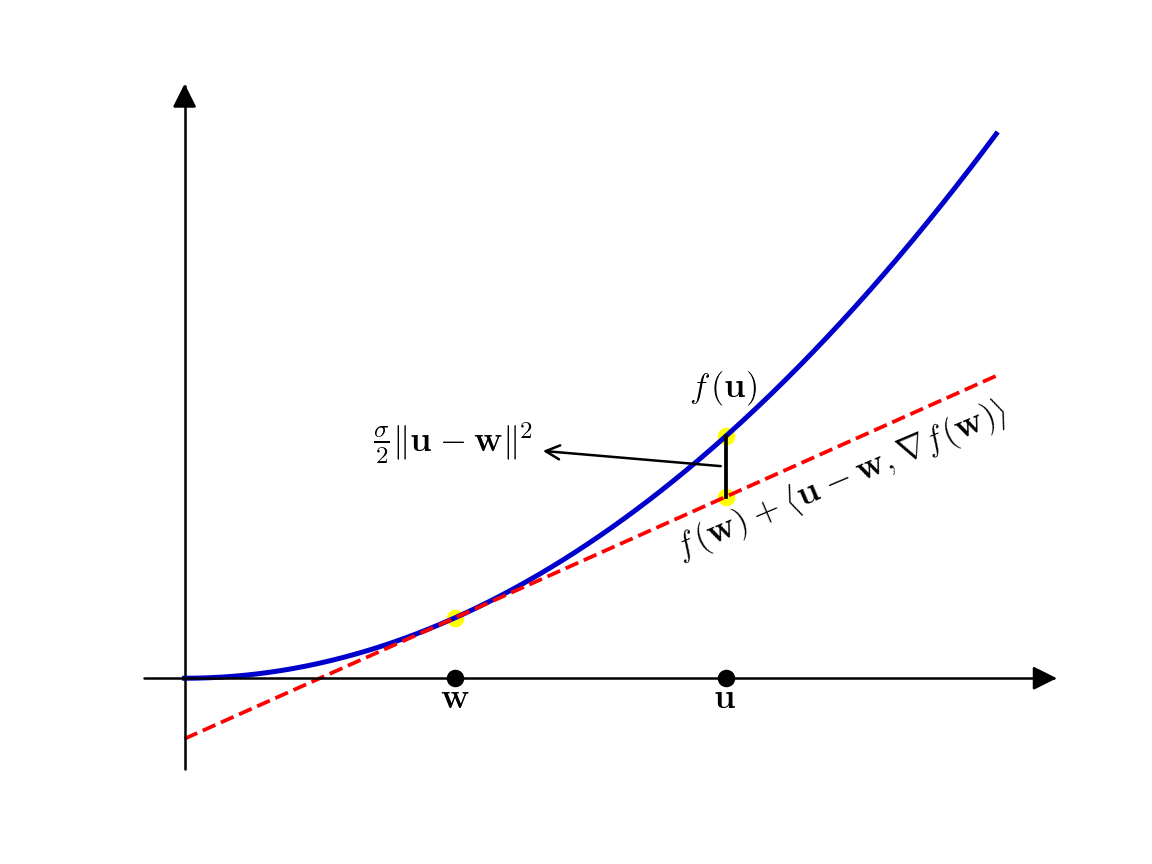
\includegraphics[width=1.8\columnwidth]{figure/newton fig2.png}
 \end{center}
  %%%
\end{minipage}



\end{frame}

\begin{frame}[fragile]
\frametitle{牛顿法分析:近似}


 考虑函数 $f(x)$的二次近似:
$$
    \phi_2(x) = f(\bar{x}) + \langle f'(\bar{x}), x-\bar{x}\rangle + \frac{1}{2} \langle f''(\bar{x})(x-\bar{x}), x-\bar{x}\rangle.
$$
$\rightarrow$ 该二次函数的最小值点是
$$
    x_2^* = \bar{x}-[f''(\bar{x})]_{}^{-1} f'(\bar{x}),
$$
这正是牛顿法的迭代公式.



\end{frame}

\begin{frame}[fragile]
\frametitle{牛顿法分析:近似}


 考虑函数 $f(x)$的二次近似:
$$
    \phi_2(x) = f(\bar{x}) + \langle f'(\bar{x}), x-\bar{x}\rangle + \frac{1}{2} \langle f''(\bar{x})(x-\bar{x}), x-\bar{x}\rangle.
$$
$\rightarrow$ 该二次函数的最小值点是
$$
    x_2^* = \bar{x}-[f''(\bar{x})]_{}^{-1} f'(\bar{x}),
$$
这正是牛顿法的迭代公式.



\end{frame}


\begin{frame}[allowframebreaks]
\frametitle{另一种解释}



%  Let us provide it with one more interpretation.

\begin{itemize}
  \item
非线性函数$f(x)$矩阵的梯度和Hessian是关于标准欧几里得内积在$R^n$定义的:
$$
    \langle x,y\rangle = \sum_{i=1}^n x_i y_i, \quad x,y\in R^n,\quad \|x\|=\langle x,x\rangle_{}^{1/2}.
$$
实际上,梯度的定义是
$$
    f(x+h) = f(x) + \langle f'(x),h\rangle + o(\|h\|),
$$
%and from this equation we derive its coordinate representation:
%$$
%    f'(x) = \left( \frac{\partial f(x)}{\partial x_1}, \cdots, \frac{\partial f(x)}{\partial x_n} \right)_{}^T.
%$$

\item  \hint{现在介绍一种新的内积.}
假设矩阵$A$为 $n\times n$ 阶正定矩阵.对于 $x,y\in R^n$ 记
\red{
$$
    \langle x,y \rangle_{A}^{} = \langle Ax,y\rangle, \quad \|x\|_A^{} = \langle Ax,x\rangle_{}^{1/2}.
$$
}

\item 函数 $\|x\|_{A}^{}$ 是 $R^n$上的一个范数.
 \footnotehint{ 这个新范数与欧式范数等价:}
$$
    \lambda_n(A)_{}^{1/2}\|x\|\leq \|x\|_A \leq \lambda_1^{}(A)_{}^{1/2} \|x\|,
$$
其中$\lambda_n(A)$ 和 $\lambda_1^{}(A)$ 是矩阵$A$的最小特征值和最大特征值.


\dred{ 使用新的内积计算的梯度和Hessian矩阵发生了改变:
$$
\begin{aligned}
   f(x+h) & = f(x) + \langle f'(x),h\rangle + \frac{1}{2} \langle f''(x)h,h \rangle + o(\|h\|^2) \\
          & = f(x) + \langle A_{}^{-1}f'(x),h\rangle_{A}^{} + \frac{1}{2} \langle A_{}^{-1}f''(x)h,h \rangle_{A}^{} + o(\|h\|^2) \\
   \end{aligned}
$$
}


\item[] $\Rightarrow$
\hint{$ f_{A}^{\prime}(x) \stackrel{\triangle}{=} A_{}^{-1}f'(x)$ 是新的梯度, 
$f_{A}^{\prime\prime}\stackrel{\triangle}{=} A_{}^{-1}f''(x)$ 是新的Hessian矩阵.
}

\item[]
\hint{ 牛顿法的下降方向可以视为$A=f''(x)$定义的度量下的梯度方向.}

\item \footnotehint{相对于 $A = f''(x)$ 计算的$f(x)$在 $x$ 处的Hessian矩阵为单位矩阵$I_n$. }

\end{itemize}

\end{frame}

\begin{frame}[fragile]
\frametitle{示例:二次函数牛顿法的一步收敛}

\begin{example}[示例]\label{eg_1_3_1}
%\textbf{For a quadratic function the Newton method converges in one step}
    考虑二次函数
    $$
        f(x) = \alpha + \langle x,x\rangle + \frac{1}{2}\langle Ax,x\rangle,
    $$
    其中 $A=A_{}^{T}\succ 0$. 因此$f'(x) = Ax+a$, $f''(x) = A$ 令
    $$
        f'(x^*) = Ax^* + a = 0
    $$
    得 $x^*  = -A_{}^{-1}a$.
    计算牛顿方向   $x\in R^n$:
    $$
        d_N(x) = [f''(x)]_{}^{-1}f'(x) = A_{}^{-1}(Ax+a) = x + A_{}^{-1}a.
    $$
    $\Rightarrow$ 对于任意的 $x\in R^n$, $x-d_N(x) = - A_{}^{-1}a = x^*$.
    \hint{$\Rightarrow$ 对于二次函数,牛顿法迭代一步即可收敛.}
    %Note also that
    \footnotehint{
    $$
        \begin{aligned}
            f(x) & = \alpha + \langle A_{}^{-1}a,x\rangle_A^{} + \frac{1}{2}\|x\|_{A}^2,\\
            f_{A}^{\prime}(x) & = A_{}^{-1} f'(x) = d_N^{}(x), %\\
            \qquad
            f_{A}^{\prime\prime}(x)   = A_{}^{-1}f''(x) = I_n.\\
        \end{aligned}
    $$
    }
\end{example}


\end{frame}

\section{拟牛顿法}

\begin{frame}[fragile]
\frametitle{拟牛顿法}

 \hint{可以尝试使用函数$f(x)$的其他近似方法, 这些方法比$\phi_1(x)$ 近似程度更好,而且比$\phi_2(x)$}的计算代价更少.


设 $G$ 为一个正定的$n\times n$阶矩阵.
有
$$
    \phi_{G}^{}(x) = f(\bar{x}) + \langle f'(\bar{x},x-\bar{x}\rangle + \frac{1}{2} \langle G(x-\bar{x}), x-\bar{x}\rangle.
$$
为了计算其最小值点,令
$$
    \phi_{G}^{\prime}(x) = f'(\bar{x}) + G(x_{G}^{*}- \bar{x}) =0,
$$
我们得到
\begin{equation}\label{EQ_1_3_1}
    x_{G}^{*} = \bar{x}-G_{}^{-1}f'(\bar{x}).
\end{equation}
\dred{若序列满足
$$
    \{G_k\}: \ G_k \longrightarrow f''(x^*)
$$
(或 $\{H_k\}:\quad H_k\equiv G_k^{-1}\rightarrow [f''(x^*)]_{}^{-1}$, 称为变尺度方法或拟牛顿方法.}
\footnotehint{在这些方法中,生成序列的过程中只涉及梯度
$\{G_k\}$ 或 $\{H_k\}$.}

更新规则 (4):
 \hint{$x_{G}^{*} = \bar{x}-G_{}^{-1}f'(\bar{x})$,}
  在优化算法中非常常见.

\end{frame}


\begin{frame}[fragile]
\frametitle{变尺度法}

%Let us write sown a general scheme of the \textit{variable metirc} method.

\myfbox{0.95\textwidth}{%
    \begin{center}
    \textbf{变尺度法}
    \end{center}
\begin{enumerate}
\item[0.] 设 $x_0 \in R^n$. 令 $H_0 = I_n$.
计算 $f(x_0)$ 和 $f'(x_0)$.


\item[1.] 第$k$次迭代 ($k\geq0$).
    \begin{enumerate}
    \item[(a)] 设 $p_k = H_k f'(x_k)$.
    \item[(b)]  $x_{k+1}= x_k - h_kp_k$
    \item[(c)] 计算 $f(x_{k+1}^{})$ and $f'(x_{k+1})$.
    \item[(d)] 更新矩阵 $H_k: H_k\rightarrow H_{k+1}^{}$.
    \end{enumerate}
\end{enumerate}
}%

\footnotehint{
\begin{itemize}
  \item
不同的变尺度法区别:
步骤的实施 1(d)

\item 步骤 1(d):  更新   $H_k$ $\leftarrow$  梯度 $+$ 函数值  %    values $f'(x_{k+1}^{})$.

\end{itemize}
}


\end{frame}

\begin{frame}[fragile]
\frametitle{拟牛顿公式: 如何构造 $H_{k+1}$ 以近似 $f''(x_{k+1})^{-1}$? }

\hint{假设 $H_{k}$ 以近似 $f''(x_{k})^{-1}$ }

\begin{itemize}
	\item Motivation\,1. \hint{函数$f(x)$在$x=x_{k+1}$处的二阶近似:}

$f(x) \approx f(x_{k+1}) + \langle f'(x_{k+1}),x-x_{k+1}\rangle 
+ \frac{1}{2} (x-x_{k+1})^{T} f''(x_{k+1}) (x-x_{k+1})$

$\rightarrow$ $f'(x) \approx    f'(x_{k+1}) 
+     f''(x_{k+1}) (x-x_{k+1})$ 

%	$\phi(x+\Delta x) \approx \phi(x) + [\phi'(x)]^{T} \Delta x$

%令 $\phi(x) =f'(x) $ $\rightarrow$	 	$f'(x+\Delta x) \approx f'(x) + [f''(x)]^{T} \Delta x$

 

%令 $ x \rightarrow x_k   $,  $\Delta x = x_{k+1} - x_k$ 
 令 $ x = x_k   $,  $f''(x_{k+1}) \approx H_{k+1}$
     $\rightarrow$	 
  $  H_{k+1}^{} (f'(x_{k+1}^{}) - f'(x_k) ) =  x_{k+1}^{}- x_{k}^{} $   
	
\item Motivation\,2. \hint{二次函数的性质:}
$$
    f(x) = \alpha + \langle a,x\rangle + \frac{1}{2}\langle Ax,x\rangle,
    \quad f'(x) = Ax+a.
$$
$\Rightarrow$ 对于任意 $x,y \in R^n$,
$f'(x)-f'(y) = A(x-y)$.


\end{itemize}

%这个恒等式解释了所谓的 \hint{拟牛顿公式}的起源.
\myfbox{0.7\textwidth}{%
    \begin{center}
    \textbf{拟牛顿公式}
    \end{center}
选择$H_{k+1}$ 满足:
$$
    H_{k+1}^{}(f'(x_{k+1}^{}) - f'(x_k)) = x_{k+1}^{}- x_{k}^{}
$$
}%


%\begin{remark}[评述]
%	  \begin{itemize}
%    \item  有许多方法可以满足这种关系.
%\item   我们给出了几个最有效的方案的例子.
%
%  \end{itemize}
%\end{remark}

\end{frame}




\begin{frame}[fragile]
\frametitle{拟牛顿公式}

\begin{example}[示例]\label{eg_1_3_2}
%\textbf{Quasi-Newton update rules}
记
$$
    \Delta H_k = H_{k+1}^{} - H_{k}^{}, \quad \gamma_k = f'(x_{k+1}^{}) - f'(x_k), \quad \delta_k = x_{k+1}^{}-x_k.
$$
 一些经典的拟牛顿法:% 满足以下准则 
\begin{enumerate}
\item Rank-one correlation scheme.
  $$
    \Delta H_k = \frac{(\delta_k-H_k\gamma_k)(\delta_k-H_k\gamma_k)_{}^{T}}{\langle \delta_k-H_k\gamma_k,\gamma_k \rangle}.
  $$
\item Davidon-Fletcher-Powell scheme (DFP).
    $$
    \Delta H_k = \frac{\delta_k \delta_k^{T}}{\langle \gamma_k,\delta_k\rangle }
        -  \frac{ H_k\gamma_k \gamma_k^T H_k  }{\langle H_k\gamma_k,\gamma_k \rangle}.
  $$
\item Broyden-Fletcher-Goldfarb-Shanno scheme (BFGS).
    $$
    \Delta H_k = \frac{ H_k \gamma_k \delta_k^{T} + \delta_k\gamma_k^T H_k}{\langle H_k\gamma_k,\gamma_k  \rangle }
        -  \beta_k \frac{ H_k\gamma_k \gamma_k^T H_k  }{\langle H_k\gamma_k,\gamma_k \rangle},
  $$
  其中 $\beta_k = 1+ \langle \gamma_k,\delta_k \rangle / \langle H_k \gamma_k ,\gamma_k \rangle$.
\end{enumerate}
\hint{从计算角度来看,BFGS被认为是最稳定的方案. }
\end{example}

%Clearly, there are many other possibilities.

%\red{Question. Why BFGS is stable in practical computations?}
\end{frame}

%\begin{frame}[fragile]
%\frametitle{Rank-one correlation scheme}
%令$\Delta H_k = v_k v_k^{T}$,其中$v_k$是列向量且$v_k\neq0$,$v_k v_k^{T}\neq0.$
%$$(\Delta H_k)^{T} = (v_k v_k^{T})^{T} = v_k v_k^{T} = \Delta H_k.$$
%$$rank(\Delta H_k) = min{rank(v_k),rank(v_k^{T})} = 1.$$
%已知$H_{k+1}=H_k+\Delta H_k,H_{k+1}\gamma_k=\delta_k.$
%将$\Delta H_k$代入可得:
%$$H_k\gamma_k+v_k v_k^{T}\gamma=\delta$$
%可计算出:
%$$v_k=\frac{\delta_k-H_k\gamma_k}{v_k^{T}\gamma_k},v_k^{T}\gamma_k=\frac{\langle \delta_k-H_k\gamma_k,\gamma_k \rangle}{v_k^{T}\gamma_k}.$$
%则:
%$$\Delta H_k = v_k v_k^{T} = \frac{(\delta_k-H_k\gamma_k)(\delta_k-H_k\gamma_k)_{}^{T}}{\langle \delta_k-H_k\gamma_k,\gamma_k \rangle}.$$

%\item \hint{注:在${\langle \delta_k-H_k\gamma_k,\gamma_k \rangle}>0$时才能保证$\Delta H_k$正定}
%\end{frame}


%\begin{frame}[fragile]
%\frametitle{DFP}
%假设$\Delta H_k$ 是$\delta_k$和$H_k\gamma_k$的线性组合,其中$\delta_k$和$H_k\gamma_k$是线性无关的。

%$$\Delta H_k = a\delta_k\delta_k^{T}+b(H_k\gamma_k)(H_k\gamma_k)^{T}=a\delta_k\delta_k^{T}+bH_k\gamma_k\gamma_k^{T}H_k.$$
%将$\Delta H_k$代入拟牛顿公式并化简可得:
%$$[1+b(\gamma_k^{T}H_k\gamma_k)]H_k\gamma_k+(a\delta_k\gamma_k-1)\delta_k=0$$
%由线性无关可得系数为零,解出:
%$$a=\frac{1}{\langle \gamma_k,\delta_k\rangle },b=-\frac{1}{\langle H_k\gamma_k,\gamma_k \rangle}$$  
%则:
%$$\Delta H_k =\frac{\delta_k \delta_k^{T}}{\langle \gamma_k,\delta_k\rangle }
%        -  \frac{ H_k\gamma_k \gamma_k^T H_k  }{\langle H_k\gamma_k,\gamma_k \rangle}$$
%\end{frame}


%\begin{frame}[fragile]
%\frametitle{DFP算法的正定性及二次终止性}
%\begin{itemize}
%\item \textbf{正定性}
%若$f'(x_k)\neq0(i=1,2,…,n)$,则DPF方法构造的矩阵$H_i(i=1,2,…,n)$为对称正定矩阵.




%\item \textbf{二次终止性 }

%若目标函数为正定二次函数,则DFP方法经有限步必达到极小点。即具有二次终止性。

%\end{itemize}

%\end{frame}

%\begin{frame}[fragile]
%\frametitle{BFGS}
%\begin{figure}[!t]
%    \centering
%    
\includegraphics[width=0.8\textwidth]{sec5-3-Newton method/small-member/SMaLL.jpg}
%    \label{fig:enter-label}
%\end{figure}
%\hint{从计算角度来看,BFGS被认为是最稳定的方案. }
%\end{frame}

\begin{frame}{拟牛顿法另一解释}
拟牛顿法与梯度下降法有相似迭代格式:
\begin{equation}\label{EQ_1_3_1}
    x_{k+1}=x_k+\alpha_kd_k
\end{equation}
\begin{equation}\label{EQ_1_3_1}
    d_k=-D_k\nabla f(x_k).
\end{equation}   
其中$D_k$是正定矩阵。可以不断校正矩阵$D_k$,使方向$d_k$趋近于牛顿方向。
\end{frame}


\begin{frame}{矩阵$D_k$的更新公式}
在最流行的一类拟牛顿算法中,矩阵$D_{k+1}$是由$\delta_k$和$\gamma_k$通过如下公式计算得到的
\begin{equation}\label{EQ_1_3_1}
    D_{k+1}=D_k+\frac{\delta_k\delta_k^{T}}{\delta_k^{T}\gamma_k}-\frac{D_k\gamma_k\gamma_k^{T}D_k}{\gamma_k^{T}D_k\gamma_k}+\xi_k\tau_kv_kv_k^{T}
\end{equation} 
其中
$$v_k=\frac{\delta_k}{\delta_k^{T}\gamma_k}-\frac{D_k\gamma_k}{\tau_k}$$
$$\tau_k=\gamma_k^{T}D_k\gamma_k$$

标量$\xi_k$满足:对于任意的$k$,
$0 \leq \xi_k \leq 1,$$D_0$是任意正定矩阵。

如果对于所有的$k$,$\xi_k=0$,我们得到Davidon-Fletcher-Powell scheme (DFP)方法。

如果对于所有的$k$,$\xi_k=1$,我们得到Broyden-Fletcher-Goldfarb-Shanno scheme (BFGS)方法。
\end{frame}

\begin{frame}
\begin{theorem}[命题]
    如果$D_k$是正定的且步长$\alpha_k$满足:
    \begin{equation}\label{EQ_1_3_1}
    \nabla f(x_k)'d_k<\nabla f(x_{k+1})'d_k
    \end{equation}
    那么由($7$)式给定的$D_k$是正定的。
\end{theorem}    
\hint{注意:}如果$x_k$不是驻点,那么有$\nabla f(x_k)'d_k<0$,因此为了满足条件($8$),执行线搜索得到满足以下条件的点$x{k+1}$就足够了。
$$|\nabla f(x_k)'d_k|<|\nabla f(x_{k+1})'d_k|$$
\hint{特别的,}如果$\alpha_k$是由最小化线搜索规则确定的,有$\nabla f(x_k)'d_k=0$且($8$)式成立。
\end{frame}

\begin{frame}
\begin{theorem}[命题]
    设{$x_k$},{$d_k$}和{$D_k$}是拟牛顿算法$(5)-(7)$式生成的序列,将其应用于正定二次函数的极小化
    $$f(x)=\frac{1}{2}x'Qx-b'x$$
    其中$\alpha_k$由下面的公式决定
    $$f(x_k+\alpha_kd_k)=\min_{\alpha}f(x_k+\alpha d_k)$$
    假设向量$x_0,…,x_{n-1}$是迭代产生的最优解,则有
    \begin{enumerate}
        \item 向量$d_0,…,d_{n-1}$是$Q$共轭的
        \item 有$D_n=Q^{-1}$
    \end{enumerate}
    
    
\end{theorem}    

\end{frame}

\begin{frame}[fragile]
\frametitle{}
\begin{itemize}
\item \textbf{超线性局部收敛速度}

%Note that for quadratic functions the variable metric methods usually terminate in $n$ iterations.
在严格最小值附近,有超线性收敛速度:
对于任意 $x_0\in R^n$ 存在 $N$ 对于所有的 $k\geq N$ 有
$$
    \|x_{k+1}^{}-x^*\| \leq \textnormal{const}\cdot \|x_k - x^*\| \cdot \|x_{k-n}^{} - x^*\|
$$
\footnotehint{ (证明过程很长)}
%As far as global convergence is concerned, these methods are not better than the gradient method
%(at least, from the theoretical point of view).



\item \textbf{需要存贮 $n\times n$矩阵 }

%在变尺度方案中,有
拟牛顿法需要 存储和更新对称的$n\times n$矩阵
$\rightarrow$ 需要\hint{$O(n^2)$} 
辅助算术运算\dred{(变尺度方法的主要缺点) }
  $\rightarrow$\textit{共轭梯度法}
%which have much lower complexity of each iteration (see Section 1.3.2).
%However, in view of an amazing growth of computer power in the last decades, these objections
%are not so important anymore.
\end{itemize}

\end{frame}


    

\begin{frame}[allowframebreaks]
  \frametitle{作业}
  
  \begin{enumerate}
  	\item (选作) 基于牛顿法 设计求 $a^{1/3}$ 的快速迭代算法,其中 $a>0$. 
  	\item 	编程题:第1部分第1节中,有练习题: 自行选取二分类数据集,编程实现 梯度下降法 求解Logistic 回归模型,并对数据集进行分类,计算分类准确率。
  	请 在此基础上,分别使用  (阻尼)牛顿法 
  	和 BFGS 方法 确定每一次迭代的步长。 
  	
  	\item 
  基于以下方法编程求解 $\min_x f(x)$
  (1) 梯度下降法;
  (2) (阻尼)牛顿法;
  (3) BFGS 方法(选作)

  \begin{enumerate}
    \item   $    f(x)=\frac{1}{2} x^{T} A x-b^{T} x$,

    其中 $A=\operatorname{diag}(20,10,2,1), \quad b=(1,1,1,1)^{T}$.

初始点 $x_{0}=(0,0,0,0)^{T}$;
最佳解决方案  $x^{*}=(0.05,0.1,0.5,1)^{T}$;
最优值 $f^{*}=0.8250$.



\item  $  f=\sum_{i=1}^{N / 2}\left[\left(x_{2 i}-x_{2 i-1}^{2}\right)^{2}+\left(1-x_{2 i-1}\right)^{2}\right]$


初始点 $x_{0}=(-1.2,1,-1.2,1, \ldots,-1.2,1)^{T} ;$
	最优解  $x^{*}=(1,1, \ldots, 1)^{T} ;$
最优值  $f^{*}=0$.
 
 
 \item  \hint{(选作)}  [扩展 Dixon 函数]
 
 $$
  f(x)=\sum_{i=1}^{n / 10}\left[\left(1-x_{10 i-9}\right)^{2}+\left(1-x_{10 i}\right)^{2}+\sum_{j=10 i-9}^{10 i-1}\left(x_{j}^{2}-x_{j+1}\right)^{2}\right]
$$

初始点 $x_{0}=(-2,-2, \cdots,-2)^{T}$; 
最佳解决方案 $x^{*}=(1,1, \cdots, 1)^{T}$; 
 最优值 $f^{*}=0$.

  \end{enumerate}


\end{enumerate}
\end{frame}


 

%\end{CJK*}
\end{document}



